
\chapter{생존분석}

{\bf 생존분석(Survival analysis)}은 무언가 얼마나 지속하는지를 기술하는 방법이다. 종종 사람 생명 연구에 사용되지만, 또한 기계나 전자 부품의 ``생존(survial)'' 혹은 좀더 일반적으로 사건 전 시간 간격에도 적용된다.
\index{생존분석 (survival analysis)}
\index{기계 부품 (mechanical component)}
\index{전자 부품 (electrical component)}

만약 여러분이 알고 있는 누군가 생명을 위협하는 질병을 진단받았다면, ``5년 생존율 (5-year survival rate)''을 들어봤을지도 모른다. 진단 후에 5년을 생존할 확률이다. 이 추정값과 관련된 통계량이 생존분석 결과다.
\index{생존율 (survival rate)}

이번 장에서 사용되는 코드는 {\tt survival.py}에 있다.
코드를 다운로드하고 작업하는 것에 대한 정보는 ~\ref{code}을 참조한다.


\section{생존곡선 (Survival curves)}
\label{survival}

생존분석에 기본 개념은 {\bf 생존곡선 (survival curve)} $S(t)$로,
존속 $t$를 $t$보다 더 오래 생존할 확률로 매핑하는 함수다.
만약 존속(duration) 분포 즉, ``수명(lifetimes)''을 알고 있다면,
생존곡선을 찾는 것은 쉽다; CDF의 여분포(complement)가 된다.
\index{생존곡선 (survival curve)}
%
\[ S(t) = 1 - \CDF(t) \]
%
여기서, $CDF(t)$는 $t$보다 적거나 같은 수명 확률이다.
\index{상보 CDF (complementary CDF)} 
\index{CDF!상보(complementary)} 
\index{CCDF}

예를 드어, NSFG 데이터셋에서 11189 출산 존속기간을 알고 있다.
이 데이터를 읽어서 CDF를 계산할 수 있다.
\index{임신기간 (pregnancy length)}

\begin{verbatim}
    preg = nsfg.ReadFemPreg()
    complete = preg.query('outcome in [1, 3, 4]').prglngth
    cdf = thinkstats2.Cdf(complete, label='cdf')
\end{verbatim}

결과 코드(outcome code) {\tt 1, 3, 4}은 정상출산, 사산, 유산을 각각 나타낸다.
분석을 위해서 유발유산(induced abortion), 자궁외 임신(ectopic pregnancy), 그리고 응답자와 인터뷰중에 임신상태인 경우는 제외한다.

데이터프레임 메쏘드 {\tt query}는 부울 표현식을 인자로 받아서 각 행마다 평가하고 참(True)을 산출하는 행을 선택한다.
\index{데이터프레임 (DataFrame)}
\index{부울 (boolean)}
\index{쿼리 (query)}

\begin{figure}
% survival.py
\centerline{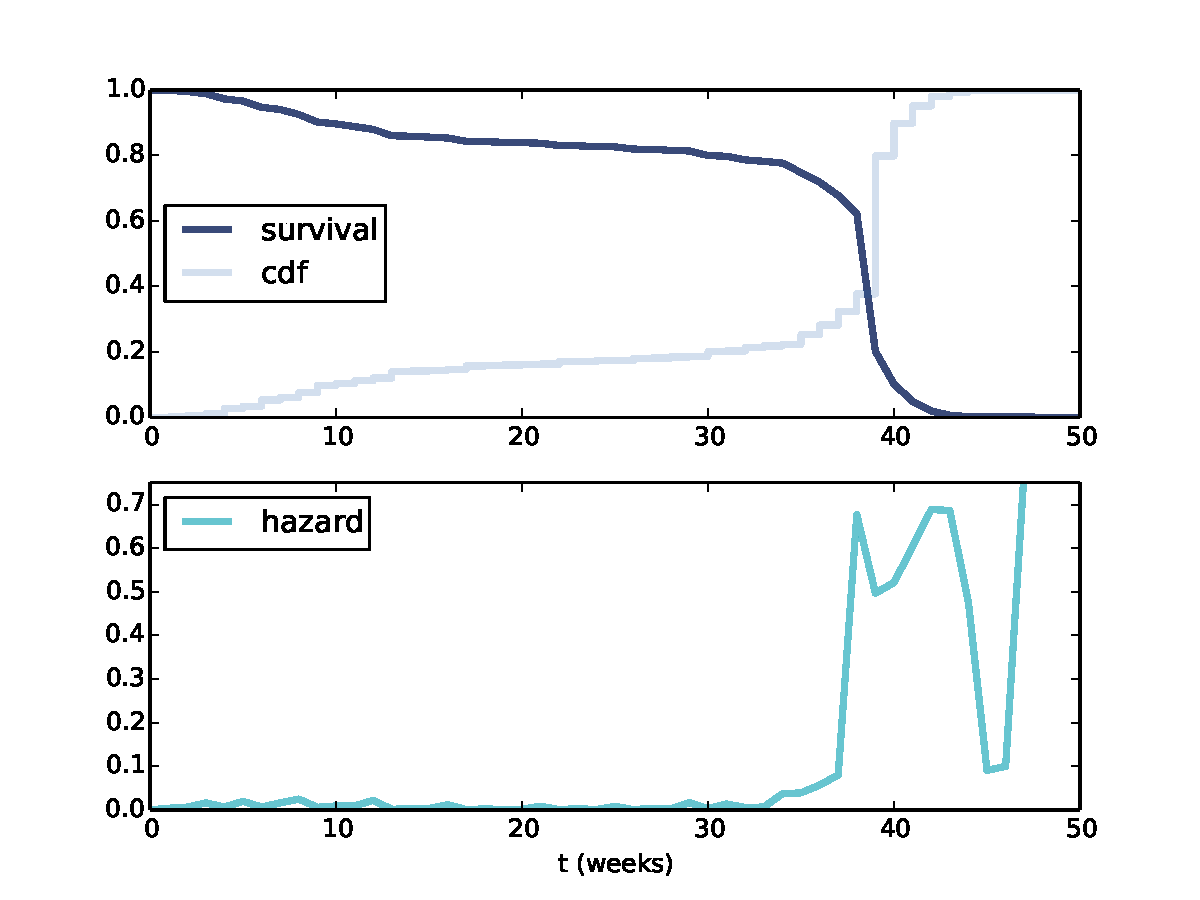
\includegraphics[height=3.0in]{figs/survival1.pdf}}
\caption{임신기간에 대한 CDF와 생존함수(위쪽), 위험함수(아래쪽).}
\label{survival1}
\end{figure}

그림~\ref{survival1} (상단)에 임신기간 CDF와 생존함수인 상보 CDF가 보여진다. 생존함수를 표현하기 위해서, 객체를 정의해서 Cdf를 래핑(wrapping) 인터페이스를 조정하여 맞춘다(adapt).
\index{Cdf}
\index{임신기간 (pregnancy length)}
\index{SurvivalFunction}

\begin{verbatim}
class SurvivalFunction(object):
    def __init__(self, cdf, label=''):
        self.cdf = cdf
        self.label = label or cdf.label

    @property
    def ts(self):
        return self.cdf.xs

    @property
    def ss(self):
        return 1 - self.cdf.ps
\end{verbatim}

{\tt SurvivalFunction}는 프로퍼티(property)를 두개 제공한다; {\tt ts}는 수명 시퀀스고, {\tt ss}는 생존함수다.
파이썬에서 ``프로퍼티(property)''는 마치 변수처럼 호출할 수 있는 메쏘드다.

수명 CDF를 인자로 넘김으로써 {\tt SurvivalFunction}를 인스터스화할 수 있다.
\index{프로퍼티 (property)}

\begin{verbatim}
    sf = SurvivalFunction(cdf)
\end{verbatim}

또한 {\tt SurvivalFunction}는 \verb"__getitem__"와 {\tt Prob}을 제공하는데 생존함수를 평가한다.

\begin{verbatim}
# class SurvivalFunction

    def __getitem__(self, t):
        return self.Prob(t)

    def Prob(self, t):
        return 1 - self.cdf.Prob(t)
\end{verbatim}

예를 들어, {\tt sf[13]} 는 임신초기 3개월을 지난 임신 비율이다.
\index{임신 3개월 (trimester)}

\begin{verbatim}
>>> sf[13]
0.86022
>>> cdf[13]
0.13978
\end{verbatim}

약 86\% 임신이 첫 3개월을 지났다; 약 14\% 그렇지 못하다.

{\tt SurvivalFunction}는 {\tt Render} 기능있다. 그래서,
{\tt thinkplot}에 함수를 사용해서 {\tt sf} 플롯을 그릴 수 있다.
\index{thinkplot}

\begin{verbatim}
    thinkplot.Plot(sf)
\end{verbatim}

그림~\ref{survival1} (상단)에 결과가 나와 있다.

곡선은 거의 13주차에서 26주차는 거의 평평해서, 임신 중기에는 임신 몇몇사례만 중단되는 것을 보여준다. 그리고, 곡선이 39주차에 가장 가파른데 가장 흔한 임신기간이다.
\index{임신기간 (pregnancy length)}


\section{위험 함수 (Hazard function)}
\label{hazard}

생존함수에서 {\bf 위험함수(hazard function)}를 도출할 수 있다; 임신기간에 대해서, 위험함수는 시간 $t$에서 t까지 계속되고 나서 t에서 끝나는 임신 비율이다. 좀더 정확하게는 다음과 같다.

%
\[ \lambda(t) = \frac{S(t) - S(t+1)}{S(t)} \]
%

분자는 $\PMF(t)$로 $t$에서 끝나는 수명 비율이다.
\index{위험함수 (hazard function)}

{\tt SurvivalFunction}는 {\tt MakeHazard} 함수를 제공하는데, 위험 함수를 계산한다.

\begin{verbatim}
# class SurvivalFunction

    def MakeHazard(self, label=''):
        ss = self.ss
        lams = {}
        for i, t in enumerate(self.ts[:-1]):
            hazard = (ss[i] - ss[i+1]) / ss[i]
            lams[t] = hazard

        return HazardFunction(lams, label=label)
\end{verbatim}

{\tt HazardFunction} 객체는 판다스 시리즈 에 대한 랩퍼다. 
\index{판다스 (pandas)}
\index{시리즈 (Series)}
\index{랩퍼 (wrapper)}

\begin{verbatim}
class HazardFunction(object):

    def __init__(self, d, label=''):
        self.series = pandas.Series(d)
        self.label = label
\end{verbatim}

{\tt d}는 딕셔너리 혹은 또다른 시리즈를 포함해서 시리즈를 초기화할 수 있는 다른 어떤 자료형도 될 수 있다. {\tt label}은 플롯으로 그림을 그렸을 때, {\tt HazardFunction}을 식별하는데 사용되는 문자열이다.
\index{HazardFunction}

{\tt HazardFunction}은 \verb"__getitem__"을 제공해서, 다음과 같이 평가할 수 있다.

\begin{verbatim}
>>> hf = sf.MakeHazard()
>>> hf[39]
0.49689
\end{verbatim}

So of all pregnancies that proceed until week 39, about
50\% end in week 39.

그림~\ref{survival1} (아래)에 임신 기간에 대한 위험함수가 보여진다.
임신 42주차 이후 시간에 대해, 위험함수가 불규칙한데, 적은 사례에 기초하기 때문이다. 그 부분을 제외하고, 곡선 모양은 예상한 것과 같다; 약 39주차에 가장 높고, 임신 중기보다 초기에 약간 더 높다.

\index{임신기간 (pregnancy length)}

위험함수는 그자체로 유용하지만, 또한 다음 절에서 살펴보듯이, 생존곡선을 추정하는데 중요한 도구가 된다.

\section{생존곡선 추정하기}

만약 누군가 여러분에게 수명 CDF를 준다면, 생존함수와 위험함수를 계산하기는 쉽다. 하지만, 많은 현실 시나리오에서, 직접 수명분포를 측정할 수는 없다.
유추해야만 한다.
\index{생존곡선 (survival curve)}
\index{CDF}

예를 들어, 진단뒤에 얼마나 오랜기간동안 환자가 생존하는지 살펴보기 위해서 한 환자집단을 추적조사한다고 가정하자.
모든 환자가 동일한 날에 진단받은 것은 아니다. 그래서 시점 아무때나 일부 환자가 다른 환자보다도 더 오래 생존한다. 만약 환자 일부가 죽는다면, 죽은 환자 생존시간을 알게된다. 여전히 살아 있는 환자에 대해서, 생존시간을 알지 못하지만, 생존시간 하한에 대한 정보는 갖게 된다.
\index{진단 (diagnosis)}

만약 모든 환자가 죽을 때까지 기다린다면, 생존곡선을 계산할 수 있다.
하지만, 새로운 처리(treatment)에 대한 효과성을 평가한다면, 그렇게 오래 기다릴 수는 없다. 불완전한 정보 (incomplete information)를 사용해서 생존곡선을 추정할 방법이 필요하다.
\index{불완전 정보 (incomplete information)}

좀더 명량한 예제로, NSFG 데이터를 사용해서 응답자가 초혼 때까지 얼마나 오래 ``생존(survive)''하는지 정량화할 것이다. 
응답자 연령 범위는 14세에서 44세까지다. 그래서, 데이터셋이 일생에서 서로다른 단계에 있는 여성의 스탭샷(snapshot) 정보를 제공한다. 

\index{결혼상태 (marital status)}

결혼한 여성에 대해서, 데이터셋에는 초혼 날짜와 그 당시 연령 정보가 포함되어 있다. 결혼하지 않은 여성에 대해서는 인터뷰했을 당시 연령정보가 있지만, 언제 혹은 결혼을 할 것인지 알 수 있는 방법이 없다.

\index{연령 (age)}

{\em 몇몇} 여성에 대한 초혼 연령을 알고 있기 때문에, 나머지를 제외하고 정보가 있는 데이터 CDF를 계산하고 싶은 유혹이 있다. 이것은 매우 바람직하지 못하다. 결과가 두가지 방향에서 잘못 도출될 수 있다; (1) 좀더 나이가 많은 여성이 더 많이 대표 표본으로 되는데, 인터뷰 당시 좀더 결혼할 것 같기 때문이다. (2) 결혼한 여성이 더 많이 대표 표본이 될 것이다. 사실, 분석 결과 모든 여성은 결혼한다는 결론이 도출될 것이다. 하지만 분명하게 틀렸다.


\section{캐플란-마이어 추정 (Kaplan-Meier estimation)}

이번 예제에서, 결혼하지 않은 여성 관측정보를 포함하는 것은 바람직할 뿐만 아니라 필요한데 이유는 생존분석에서 중심적인 알고리즘 중의 하나인 {\bf 캐플란-마이어 추정(Kaplan-Meier estimation)}과 연결되기 때문이다.
\index{캐플란-마이어 추정 (Kaplan-Meier estimation)}

일반적인 생각은 데이터를 사용해서, 위험함수를 추정하고 나서, 위험함수를 생존함수로 전환한다. 위험함수를 추정하기 위해서, 각 연령별로 다음을 고려한다. (1) 그 연령에 결혼한 여성 숫자, (2) 결혼 ``위험 상태(at risk)''에 있는 여성 숫자로 이전 연령에서 결혼하지 않은 모든 여성이 포함된다.

\index{위험함수 (hazard function)}
\index{위험 상태(at risk)}

다음에 코드가 있다.

\begin{verbatim}
def EstimateHazardFunction(complete, ongoing, label=''):

    n = len(complete)
    hist_complete = thinkstats2.Hist(complete)
    sf_complete = SurvivalFunction(thinkstats2.Cdf(complete))

    m = len(ongoing)
    sf_ongoing = SurvivalFunction(thinkstats2.Cdf(ongoing))

    lams = {}
    for t, ended in sorted(hist_complete.Items()):
        at_risk = ended + n * sf_complete[t] + m * sf_ongoing[t]
        lams[t] = ended / at_risk

    return HazardFunction(lams, label=label)
\end{verbatim}

{\tt complete}는 완벽한 관측 집단이다; 이 경우에 응답자가 결혼했을 때 연령이 된다. {\tt ongoing}은 완벽하지 못한 관측 집단이다; 이 경우에 인터뷰를 했을 때 미혼인 여성 연령이 된다.

먼저, 응답자가 결혼했을 때 연령 Hist인 \verb"hist_complete",
결혼한 여성에 대한 생존함수, \verb"sf_complete", 미혼 여성에 대한 생존함수 \verb"sf_ongoing"를 미리 계산한다.
\index{Hist}
\index{생존함수 (survival function)}

응답자가 결혼했을 때 루프는 연령을 반복한다. 
{\tt t} 각 값에 대해, {\tt t} 연령에서 결혼한 여성 숫자인 {\tt ended}가 있다. 그리고 나서 다음의 합으로 ``위험 상태(at risk)'' 여성 숫자를 계산한다.

\begin{itemize}

\item {\tt ended}, 연령 {\tt t}에서 결혼한 응답자 숫자.

\item \verb"n * sf_complete[t]", 연령 {\tt t} 뒤에 결혼한 응답자 숫자.

\item \verb"m * sf_ongoing[t]", 연령 {\tt t} 후에 인터뷰한 미혼 응답자 숫자, 그러므로 {\tt t} 시점 혹은 이전에 결혼했는지 알려지지 않았다.

\end{itemize}

시점 {\tt t}에 위험함수 추정값은 \verb"at_risk"에 대한 {\tt ended}의 비율이다.

{\tt lams}은 딕셔너리로 $t$에서 $\lambda(t)$으로 매핑한다. 
결과는 {\tt HazardFunction} 객체다.
\index{HazardFunction}


\section{결혼 곡선 (marriage curve)}

이 함수를 검정하기 위해서, 데이터 정제와 변환을 수행해야 한다.
필요한 NSFG 변수는 다음과 같다.

\index{결혼상태 (marital status)}

\begin{itemize}

\item {\tt cmbirth}: 모든 응답자에 대해서 알려진, 응답자 생년월일.
\index{생년월일 (date of birth)}

\item {\tt cmintvw}: 모든 응답자에 대해 알려진, 응답자가 인터뷰한 날짜.

\item {\tt cmmarrhx}: 알려져있고 해당되면, 응답자가 첫 혼인한 날짜.

\item {\tt evrmarry}: 만약 인터뷰 날짜 이전에 결혼했다면 1, 그렇지 않으면 0.

\end{itemize}

첫 변수 세개는 ``세기-월(century-months)'' 방식으로 부호화되었다; 즉, 1899년 12월 이후 정수형 개월 숫자. 그래서, 세기-월(century-month) 1은 1900년 1월이 된다.
\index{세기 월 (century month)}

첫째, 응답자 파일을 읽고, {\tt cmmarrhx}에 있는 타당하지 않는 값 (invalid value)을 교체한다.

\begin{verbatim}
    resp = chap01soln.ReadFemResp()
    resp.cmmarrhx.replace([9997, 9998, 9999], np.nan, inplace=True)
\end{verbatim}

그리고 나서, 혼인 당시에 각 응답자 연령과 인터뷰 당시 연령을 계산한다.
\index{NaN}

\begin{verbatim}
    resp['agemarry'] = (resp.cmmarrhx - resp.cmbirth) / 12.0
    resp['age'] = (resp.cmintvw - resp.cmbirth) / 12.0
\end{verbatim}

다음에, {\tt complete} 변수에 결혼한 여성에 대해서 결혼 당시 연령 정보를 뽑아낸다. 그리고, {\tt ongoing} 변수에 결혼하지 않은 여성에 대한 인터뷰 당시 연령 정보를 대입한다.
\index{연령 (age)}

\begin{verbatim}
    complete = resp[resp.evrmarry==1].agemarry
    ongoing = resp[resp.evrmarry==0].age
\end{verbatim}

마지막으로, 위험함수를 계산한다.
\index{위험함수 (hazard function)}

\begin{verbatim}
    hf = EstimateHazardFunction(complete, ongoing)
\end{verbatim}

그림~\ref{survival2} (위)에 추정 위험함수가 그려져 있다; 10대에는 낮고, 20대에는 더 높고, 30대에는 감소한다. 40대에 다시 증가한다. 하지만, 이것은 추정 과정의 산출물이다; ``위험 상황(at risk)'' 응답자 숫자가 감소함에 따라, 혼인한 적은 여성이 높은 추정 위험을 산출한다. 생존함수는 이러한 잡음을 부드럽게 평활한다.
\index{잡음 (noise)}


\section{생존함수 추정하기}

위험함수를 갖게 되면, 생존함수를 추정할 수 있다.
{\tt t} 시점을 지나 생존할 가망성은 줄곤 살아서 {\tt t} 시점까지 생존할 가망성이 되는데, 보수 위험함수(complementary hazard function)의 누적 곱이 된다.

%
\[ [1-\lambda(0)] [1-\lambda(1)] ... [1-\lambda(t)] \]
%

{\tt HazardFunction} 클래스는 상기 누적곱을 계산하는 {\tt MakeSurvival} 함수를 제공한다.
\index{누적곱 (cumulative product)}
\index{SurvivalFunction}

\begin{verbatim}
# class HazardFunction:

    def MakeSurvival(self):
        ts = self.series.index
        ss = (1 - self.series).cumprod()
        cdf = thinkstats2.Cdf(ts, 1-ss)
        sf = SurvivalFunction(cdf)
        return sf
\end{verbatim}

{\tt ts}는 위험 함수가 추정되는 시점 시퀀스다.
{\tt ss}는 보수 위험함수 누적곱이다. 따라서, 생존함수가 된다.

{\tt SurvivalFunction}가 구현되는 방식 때문에, {\tt ss} 보수를 계산하고, Cdf를 만들고 나서, SurvivalFunction 객체를 인스턴스화 한다.
\index{Cdf}
\index{보수CDF (complementary CDF)}


\begin{figure}
% survival.py
\centerline{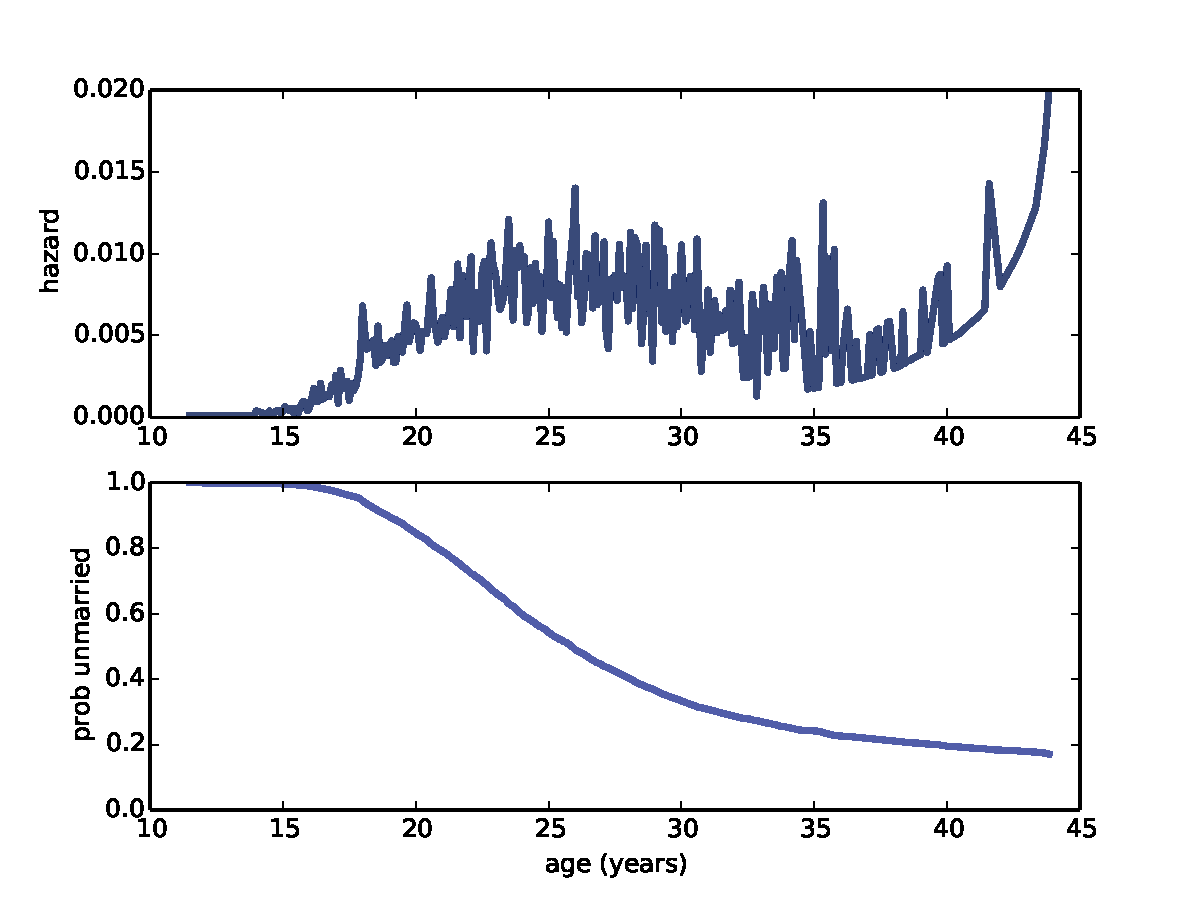
\includegraphics[height=2.5in]{figs/survival2.pdf}}
\caption{초혼 연령에 대한 위험함수(위쪽)와 생존함수(아래쪽).}
\label{survival2}
\end{figure}

그림~\ref{survival2} (아래) 에 결과가 그려져 있다.
생존곡선은 대부분의 여성이 결혼하는 25세에서 35세 사이가 가장 가파르다.
35세에서 45세 사이는 거의 평평하다. 35세 전에 결혼하지 않은 여성이 혼일할 것 같지 않다는 것을 나타낸다.

이와 같은 곡선이 1986년 유명한 잡지기사의 기초가 된다; {\it 뉴스위크(Newsweek)}에 따르면, 40세된 미혼 여성이 혼인보다도 ``테러리스트에 의해 더 살해될 가능성''이 있다. 이러한 통계량은 널리 보도되고 대중적인 문화 일부분이 되었다. 하지만, 그러고 나서 잘못되었다(왜냐하면, 오류가 있는 분석에 기반했기 때문이다) 그리고, 심지어 더 잘못된 것으로 밝혀졌다(이미 진행중이고, 지속되는 문화 변화 때문이다). 2006년 {\it 뉴스위크(Newsweek)}는 보도가 잘못되었다고 시인하는 또다른 기사를 실었다.
\index{뉴스위크 (Newsweek)}

이 기사, 기사의 기반이 된 통계량, 그리고 반응에 관해 더 읽어보기를 격려한다. 신중히 통계분석을 수행하고, 적절한 의심(appropriate skepticism)를 가지고 결과를 해석하고, 공공에게 정확하고 정직하게 제시하는데 있어, 윤리적 책임의 중요성을 상기시켰으면 한다.
\index{윤리 (ethics)}


\section{신뢰구간 (Confidence intervals)}

캐플란-마이어 분석(Kaplan-Meier analysis)은 생존곡선에 대한 단 하나의 추정값을 산출한다. 하지만, 추정값의 불확실성을 정량화하는 것도 또한 중요하다. 늘 그렇듯이, 세가지 오차 원천이 있다; 측정오차, 표집오차, 모형화 오차.

\index{신뢰구간 (confidence interval)}
\index{모형화 오차 (modeling error)}
\index{표집오차 (sampling error)}

이번 예제에서, 측정오차는 대략 작다. 일반적으로, 사람의 출생년월, 혼인여부, 혼인 시점은 알고 있다. 그리고, 이러한 정보를 정확하게 보고할 것으로 예상할 수 있다.
\index{측정 오차 (measurement error)}

재표본추출(resampling)을 통해서 표집오차를 정량화할 수 있다. 다음에 코드가 있다.
\index{재표본추출 (resampling)}

\begin{verbatim}
def ResampleSurvival(resp, iters=101):
    low, high = resp.agemarry.min(), resp.agemarry.max()
    ts = np.arange(low, high, 1/12.0)

    ss_seq = []
    for i in range(iters):
        sample = thinkstats2.ResampleRowsWeighted(resp)
        hf, sf = EstimateSurvival(sample)
        ss_seq.append(sf.Probs(ts))

    low, high = thinkstats2.PercentileRows(ss_seq, [5, 95])
    thinkplot.FillBetween(ts, low, high)
\end{verbatim}

{\tt ResampleSurvival} 함수는 응답자 데이터프레임 {\tt resp}와
재표본추출 횟수 {\tt iters}을 인자로 받는다.
{\tt ts}를 계산하는데 생존함수를 평가하는 연령 시퀀스다.
\index{데이터프레임 (DataFrame)}

루프 내부에, {\tt ResampleSurvival}는 다음과 같다:

\begin{itemize}

\item ~\ref{weighted}절에서 살펴본 {\tt ResampleRowsWeighted}을 사용해서 응답자를 재표본추출한다.
\index{가중 재표본추출 (weighted resampling)}

\item {\tt EstimateSurvival} 호출하는데, 위험곡선과 생존곡선을 추정하는데 앞절 과정을 사용한다.

\item {\tt ts}에 각 연령별로 생존곡선을 평가한다.

\end{itemize}

\verb"ss_seq"는 평가된 생존곡선 시퀀스다. 
{\tt PercentileRows}는 이 시퀀스를 받아 5번째와 95번째 백분위수를 계산하고, 생존곡선 90\% 신뢰구간을 반환한다.
\index{FillBetween}

\begin{figure}
% survival.py
\centerline{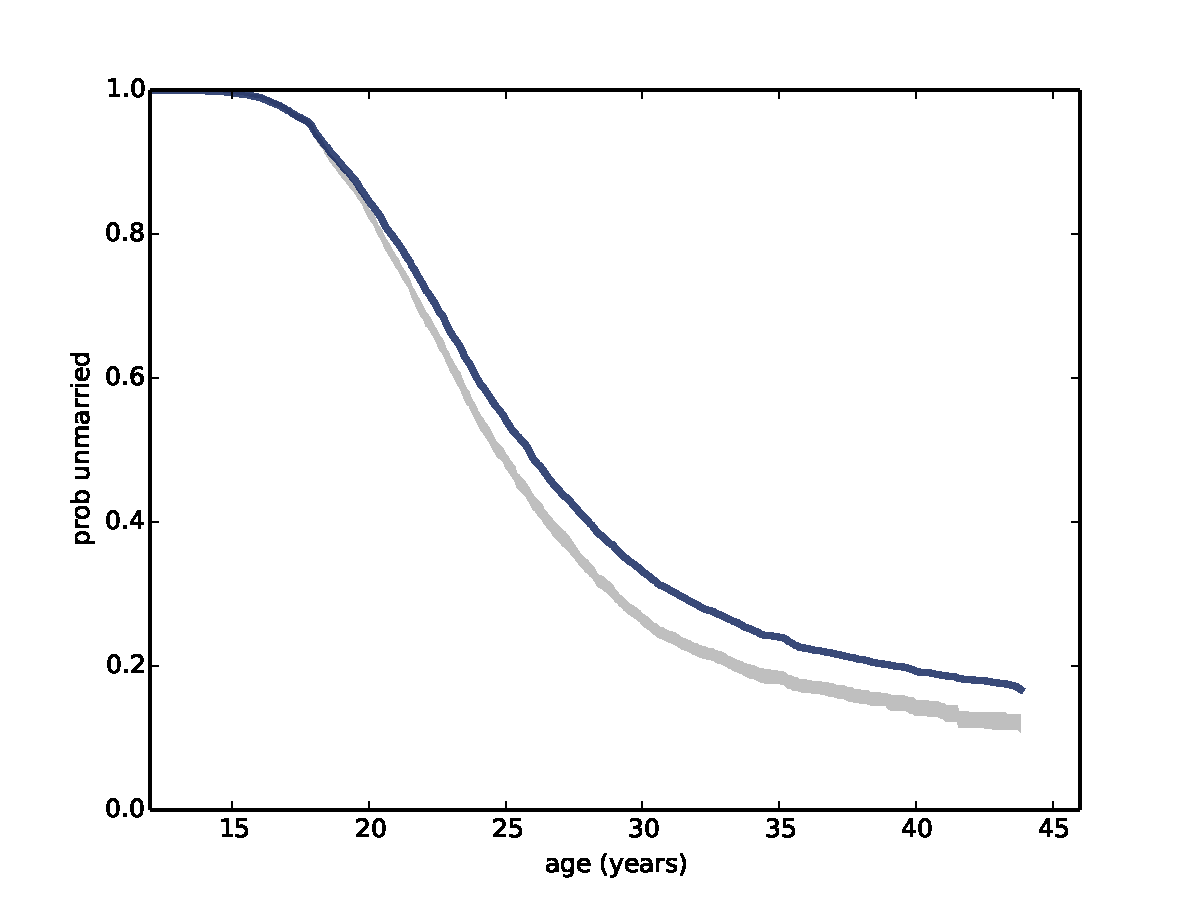
\includegraphics[height=2.5in]{figs/survival3.pdf}}
\caption{초혼연령에 대한 생존함수와 가중 재표집에 근거한 90\% 신뢰구간.}
\label{survival3}
\end{figure}

그림~\ref{survival3}에 앞절에서 추정한 생존함수와 함께 결과가 나와 있다.
신뢰구간은 추정곡선과 달리 표집 가중치(sampling weight)를 고려한다. 둘 사이에 불일치는 표집 가중치가 추정값에 상당한 효과가 있음을 나타낸다---이 사실을 유념해야 한다.
\index{신뢰구간 (confidence interval)}
\index{표집 가중치 (sampling weight)}


\section{코호트 효과 (Cohort effects)}

생존분석 도전중의 하나는 추정 곡선의 다른 부분이 응답자의 다른 집단에 기반한다는 것이다. 시점 {\tt t}에 곡선 부분은 인터뷰 당시에 적어도 응답자 연령이 적어도 {\tt t}인 응답자에 기반한다. 그래서, 곡선의 가장 왼쪽 부분은 모든 응답자로부터 데이터가 포함되어 있고, 가장 오른쪽에는 가장 나이든 응답자만 포함된다.

만약 응답자의 관련 특성이 시간에 따라 변화하지 않는다면, 문제가 되지 않고 좋다. 하지만, 이 경우에  다른 세대에 태어난 여성에 대해서 혼인 패턴은 다를 것 같다. 출생별 10년을 단위로 응답자를 집단화해서 효과를 조사할 수있다.
출생 혹은 비슷한 사건으로 정의되는 이와 같은 집단을 {\bf 코호트(cohorts)}라고 부른다. 그리고, 집단 간 차이를 {\bf 코호트 효과 (cohort effects)}라고 부른다.
\index{코호트 (cohort)}
\index{코호트 효과 (cohort effect)}

NSFG 혼인 데이터에서 코호트 효과를 조사하기 위해서, 이책 전체적으로 사용된 2002년 조사 사이클 6 데이터; ~\ref{replication}절에서 사용된 2006--2010 조사 사이클 6 데이터; 1995년 사이클 5 데이터를 수집했다. 모두 합쳐 데이터셋에는 30,769 응답자가 있다.

\begin{verbatim}
    resp5 = ReadFemResp1995()
    resp6 = ReadFemResp2002()
    resp7 = ReadFemResp2010()
    resps = [resp5, resp6, resp7]
\end{verbatim}

{\tt resp} 각 데이터프레임에 대해서, {\tt cmbirth}를 사용해서 각 응답자에 대한 출생 십년을 계산한다.
\index{판다스 (pandas)}
\index{데이터프레임 (DataFrame)}

\begin{verbatim}
    month0 = pandas.to_datetime('1899-12-15')
    dates = [month0 + pandas.DateOffset(months=cm) 
             for cm in resp.cmbirth]
    resp['decade'] = (pandas.DatetimeIndex(dates).year - 1900) // 10
\end{verbatim}

{\tt cmbirth}은 1899년 12월 이후 정수형 개월수로 부호화된다; {\tt month0}는 Timestamp 객체로 날짜를 표현한다. 각 출생일에 대해 {\tt DateOffset}를 인스턴스화하고, 세기-월을 포함하고 {\tt month0}에 더한다; 결과는 
Timestamps 시퀀스로 {\tt DateTimeIndex}로 전환된다. 마지막으로 {\tt year}를 추출하고 십년단위로 계산한다.
\index{DateTimeIndex}
\index{인덱스 (Index)}
\index{세기 월 (century month)}

표집 가중치를 고려하고, 표집오차 때문에 변동성을 보여주기 위해, 데이터를 재표본추출하고, 십년 단위로 응답자를 집단화하고, 생존곡선을 플롯으로 그린다.
\index{재표본추출 (resampling)}
\index{표집오차 (sampling error)}

\begin{verbatim}
    for i in range(iters):
        samples = [thinkstats2.ResampleRowsWeighted(resp) 
                   for resp in resps]
        sample = pandas.concat(samples, ignore_index=True)
        groups = sample.groupby('decade')

        EstimateSurvivalByDecade(groups, alpha=0.2)
\end{verbatim}

세개 NSFG 시이클 데이터는 서로 다른 표집 가중치를 사용한다. 그래서, 개별적으로 재표본추출하고 나서, {\tt concat}를 사용해서, 하나의 데이터프레임으로 병합한다. 모수 \verb"ignore_index"는 {\tt concat}에게
인덱스로 응답자를 매칭하지 못하게 한다; 대신에 0에서 30768까지 새로운 인덱스를 생성한다.
\index{판다스 (pandas)}
\index{데이터프레임 (DataFrame)}
\index{groupby}

{\tt EstimateSurvivalByDecade}는 각 코호트에 대해서 생존곡선을 플롯으로 그린다.

\begin{verbatim}
def EstimateSurvivalByDecade(resp):
    for name, group in groups:
        hf, sf = EstimateSurvival(group)
        thinkplot.Plot(sf)
\end{verbatim}

\begin{figure}
% survival.py
\centerline{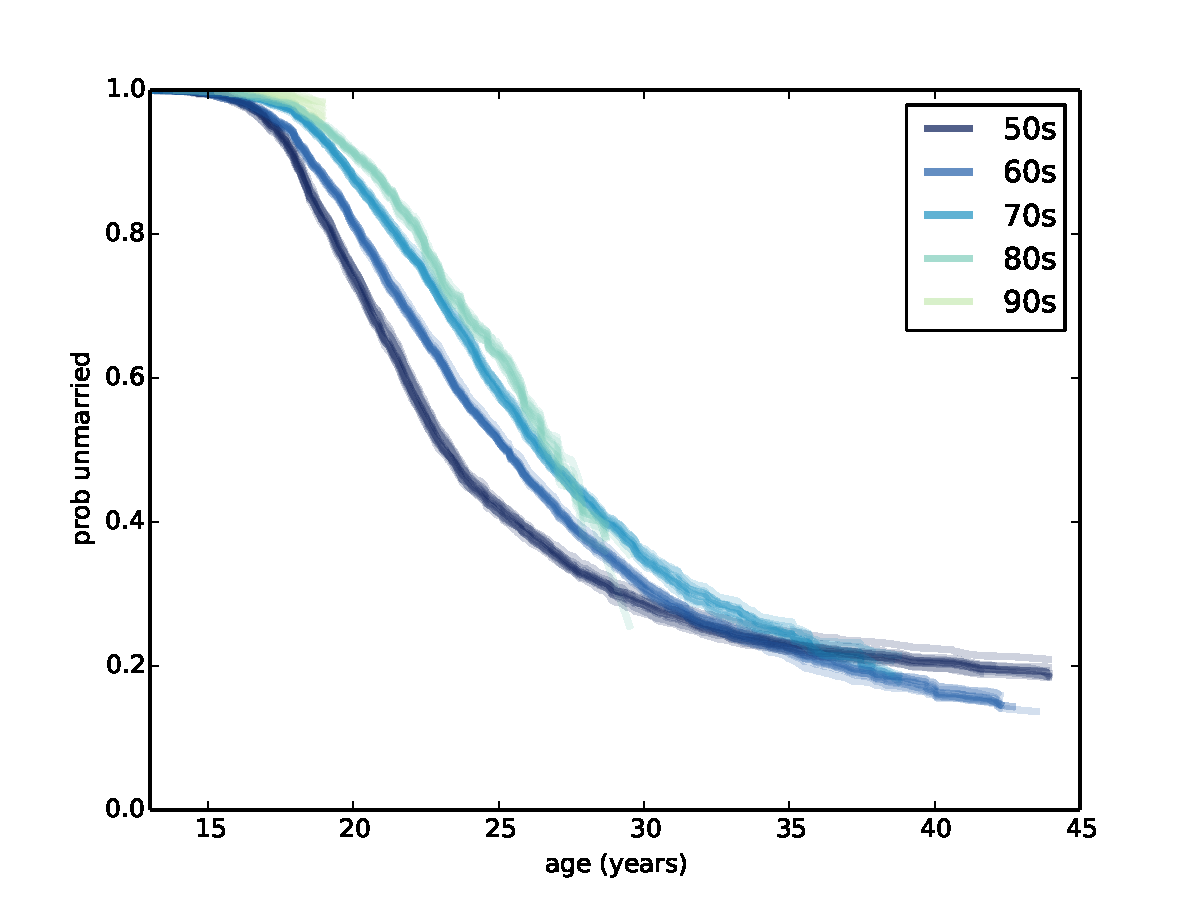
\includegraphics[height=2.5in]{figs/survival4.pdf}}
\caption{서로 다른 십년동안 출생한 응답자에 대한 생존함수.}
\label{survival4}
\end{figure}

그림~\ref{survival4}에 결과가 나와있다.
패턴 몇개가 눈에 보인다.

\begin{itemize}

\item 50년대 여성이 가장 일찍 결혼했고, 연속 코호트 혼인은 점점 늦어지고, 적어도 30대 연령까지 그렇다.

\item 60년에 태어난 여성에는 놀라운 패턴이 있다.
25세 이전에 그전 세대보다 혼인 속도가 더 늦었다. 25세 이후에는 혼인 속도가 더 빠르다. 32세경에는 50년대 코호트를 따라잡고, 44세경에는 상당히 더 결혼상태에 있을 것 같다.
\index{혼인상태 (marital status)}

60년대 태어난 여성은 1985년에서 1995년 사이 25세를 넘어선다.
앞서 언급한 {\it 뉴스위크 (Newsweek)} 기사가 1986년에 보도된 것을 기억하면, 이 기사가 결혼붐에 단초를 제공했다고 상상할 마음이 생긴다. 
이런 설명이 너무 쉬운 것이지만, 기사와 기사에 대응이 이 코호트 행동에 영향을 주었다는 기분을 나타낸다는 것도 가능하다.
\index{뉴스위크 (Newsweek)}

\item 70년대 패턴도 비슷하다. 25세 이전에 혼인하는 것이 그 전세대만 못하다. 하지만, 35세경에 이전 두세대 코호트를 모두 따라잡는다.

\item 80년생 여성은 25세전에 훨씬 덜 혼인할 것 같다. 이후에 일어난 것은 명분명하지 않다; NSFG 다음 사이틀 데이터를 기다려야만 한다.

\end{itemize}

그동안 예측도 할 수 있다.
\index{예측 (prediction)}


\section{외삽법 (Extrapolation)}

70년대생 코호트 생존곡선은 약 38세에서 끝난다; 80년대생 코호트는 약 28세에서 끝나고, 90년대생 코호트는 거의 어떤 자료도 없다.
\index{외삽법 (extrapolation)}

이전 코호트에서 데이터를 ``빌려옴(borrowing)''으로써 이들 곡선을 외삽(extrapolate)할 수 있다. 
HazardFunction에는 {\tt Extend} 메쏘드를 제공하는데, 또다른 더 긴 HazardFunction에서 꼬리를 복사한다.
\index{HazardFunction}

\begin{verbatim}
# class HazardFunction

    def Extend(self, other):
        last = self.series.index[-1]
        more = other.series[other.series.index > last]
        self.series = pandas.concat([self.series, more])
\end{verbatim}

~\ref{hazard}절에서 살펴봤듯이, HazardFunction은 $t$에서 $\lambda(t)$로 매핑하는 시리즈를 담고 있다. {\tt Extend}는 {\tt self.series}에 마지막 인덱스인 {\tt last}를 찾고, {\tt last} 다음에 오는 값을 {\tt other}에서 선택하고, {\tt self.series}에 덧붙인다.
\index{판다스 (pandas)}
\index{시리즈 (Series)}

이제 각 코호트에 대해서 이전 것에서 가져온 값을 사용해서 HazardFunction을 연장할 수 있다.

\begin{verbatim}
def PlotPredictionsByDecade(groups):
    hfs = []
    for name, group in groups:
        hf, sf = EstimateSurvival(group)
        hfs.append(hf)

    thinkplot.PrePlot(len(hfs))
    for i, hf in enumerate(hfs):
        if i > 0:
            hf.Extend(hfs[i-1])
        sf = hf.MakeSurvival()
        thinkplot.Plot(sf)
\end{verbatim}

{\tt groups}는 출생을 십년 단위로 나눈 응답자를 갖는 GroupBy 객체다.
첫번째 루프가 각 집단에 대한 HazardFunction을 계산한다.
\index{groupby}

두번째 루프가 이전 세대로부터 값(이전 집단으로부터 값을 포함할 수 있다)으로 각 HazardFunction를 연장한다.
그리고 나서, 각 HazardFunction을 SurvivalFunction로 전환하고 플롯을 그린다.

\begin{figure}
% survival.py
\centerline{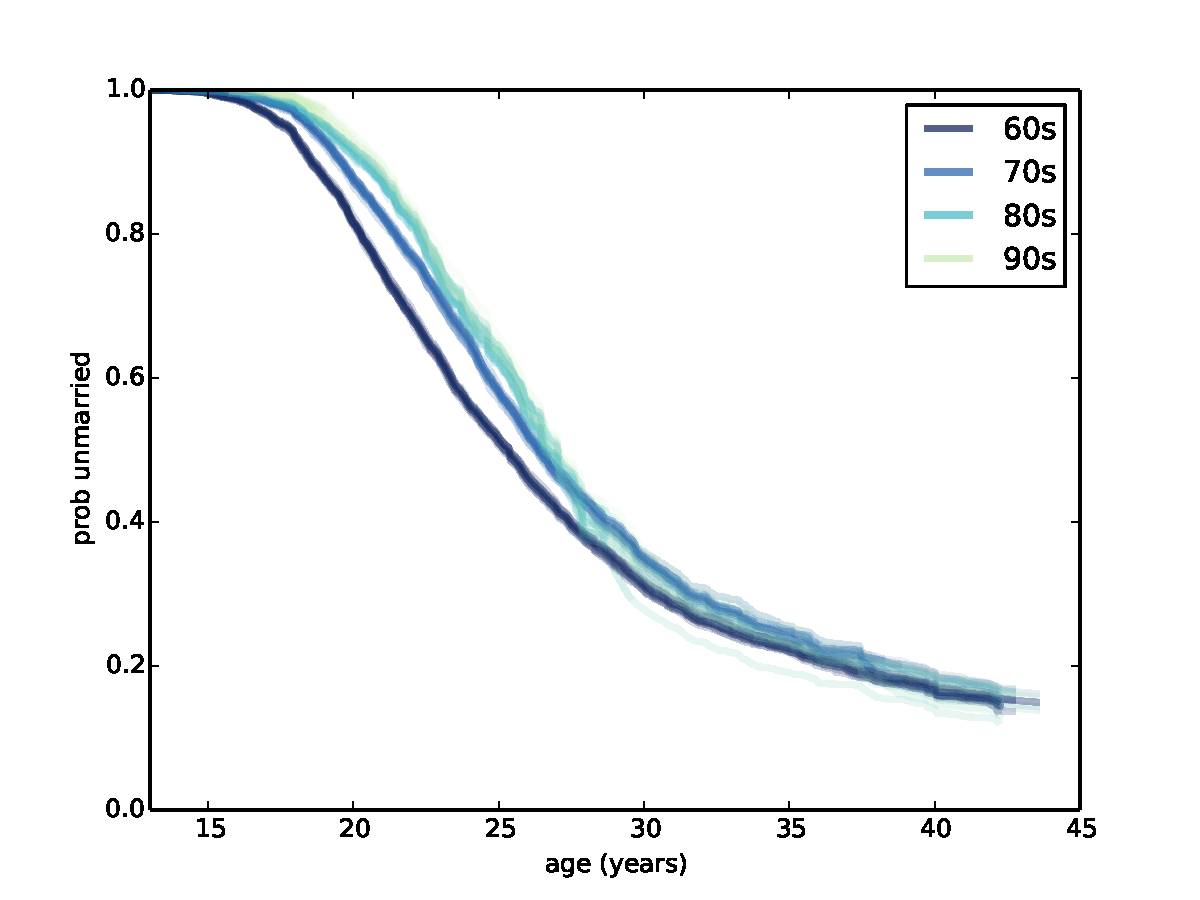
\includegraphics[height=2.5in]{figs/survival5.pdf}}
\caption{서로 다른 십년동안 출생한 응답자에 대한 생존함수와 후세 코호트에 대한 예측.}
\label{survival5}
\end{figure}

그림~\ref{survival5}에 결과가 나와있다; 50년대생 코호트를 제거해서 예측값을 좀더 가시적으로 만들었다. 이 결과가 시사하는 바는, 40세경에 가장 최신 코호트는 60대 코호트에 수렴하는데, 결코 혼인하지 않는 비율은 20\% 보다 적다.
\index{시각화 (visualization)}


\section{기대 잔존 수명}

생존곡선이 주어지면, 현재 연령 함수로 기대잔존수명을 계산할 수 있다.
예를 들어, ~\ref{survival}절에서 임신기간 생존함수가 주어지면 출산까지 예상시간을 계산할 수 있다.
\index{임신기간 (pregnancy length)}

첫단계는 수명 PMF를 추출한다. {\tt SurvivalFunction}가 이를 수행하는 메쏘드를 제공한다.

\begin{verbatim}
# class SurvivalFunction

    def MakePmf(self, filler=None):
        pmf = thinkstats2.Pmf()
        for val, prob in self.cdf.Items():
            pmf.Set(val, prob)

        cutoff = self.cdf.ps[-1]
        if filler is not None:
            pmf[filler] = 1-cutoff

        return pmf
\end{verbatim}

SurvivalFunction는 수명 Cdf를 담고 있다는 것을 기억하라. 루프가 Cdf에서 Pmf로 값과 확률을 복사한다.
\index{Pmf}
\index{Cdf}

{\tt cutoff}는 Cdf에 가장 높은 확률로, 만약 Cdf가 완전하다면 1이고, 그렇지 않다면 1보다 작다. 만약 Cdf가 불완전하다면, 완료하기 위해 제공되는 값 {\tt filler}를 꽂아 넣는다,

임신기간 Cdf는 완전하기 때문에, 아직은 이러한 세부사항까지 걱정할 필요는 없다.
\index{임신기간 (pregnancy length)}

다음 단계는 기대잔존수명을 계산하는데, 여기서 ``기대(expected)''는 평균을 의미한다.
{\tt SurvivalFunction}은 또한 이것을 수행하는 메쏘드를 제공한다.
\index{기대잔존수명 (expected remaining lifetime)}

\begin{verbatim}
# class SurvivalFunction

    def RemainingLifetime(self, filler=None, func=thinkstats2.Pmf.Mean):
        pmf = self.MakePmf(filler=filler)
        d = {}
        for t in sorted(pmf.Values())[:-1]:
            pmf[t] = 0
            pmf.Normalize()
            d[t] = func(pmf) - t

        return pandas.Series(d)
\end{verbatim}

{\tt RemainingLifetime}는 인자로 {\tt MakePmf}에 전달되는 {\tt filler}와, 
잔존수명 분포를 요약하는데 사용되는 함수 {\tt func}을 인자로 받는다.

{\tt pmf}는 SurvivalFunction에서 추출된 수명 Pmf다.
{\tt d}는  현재 연령 {\tt t}에서 기대잔존수명으로 매핑 결과를 담고 있다.
\index{Pmf}

루프가 Pmf에 값을 반복 돌린다. {\tt t} 각 값에 대해, 수명이 {\tt t}를 초과한 것을 둔 상태에서, 수명 조건부분포를 계산한다.
Pmf에서 값을 한번에 하나씩 제거하고, 남은 값을 다시 정규화함으로써 이것을 수행한다.

그리고 나서, {\tt func}를 사용해서, 조건부분포를 요약한다.
상기 예제에서, 기간이 {\tt t}를 초과했을 때 결과는 평균임신기간이 된다.
{\tt t}를 빼서, 평균잔존임신기간을 얻는다.
\index{임신기간 (pregnancy length)}

\begin{figure}
% survival.py
\centerline{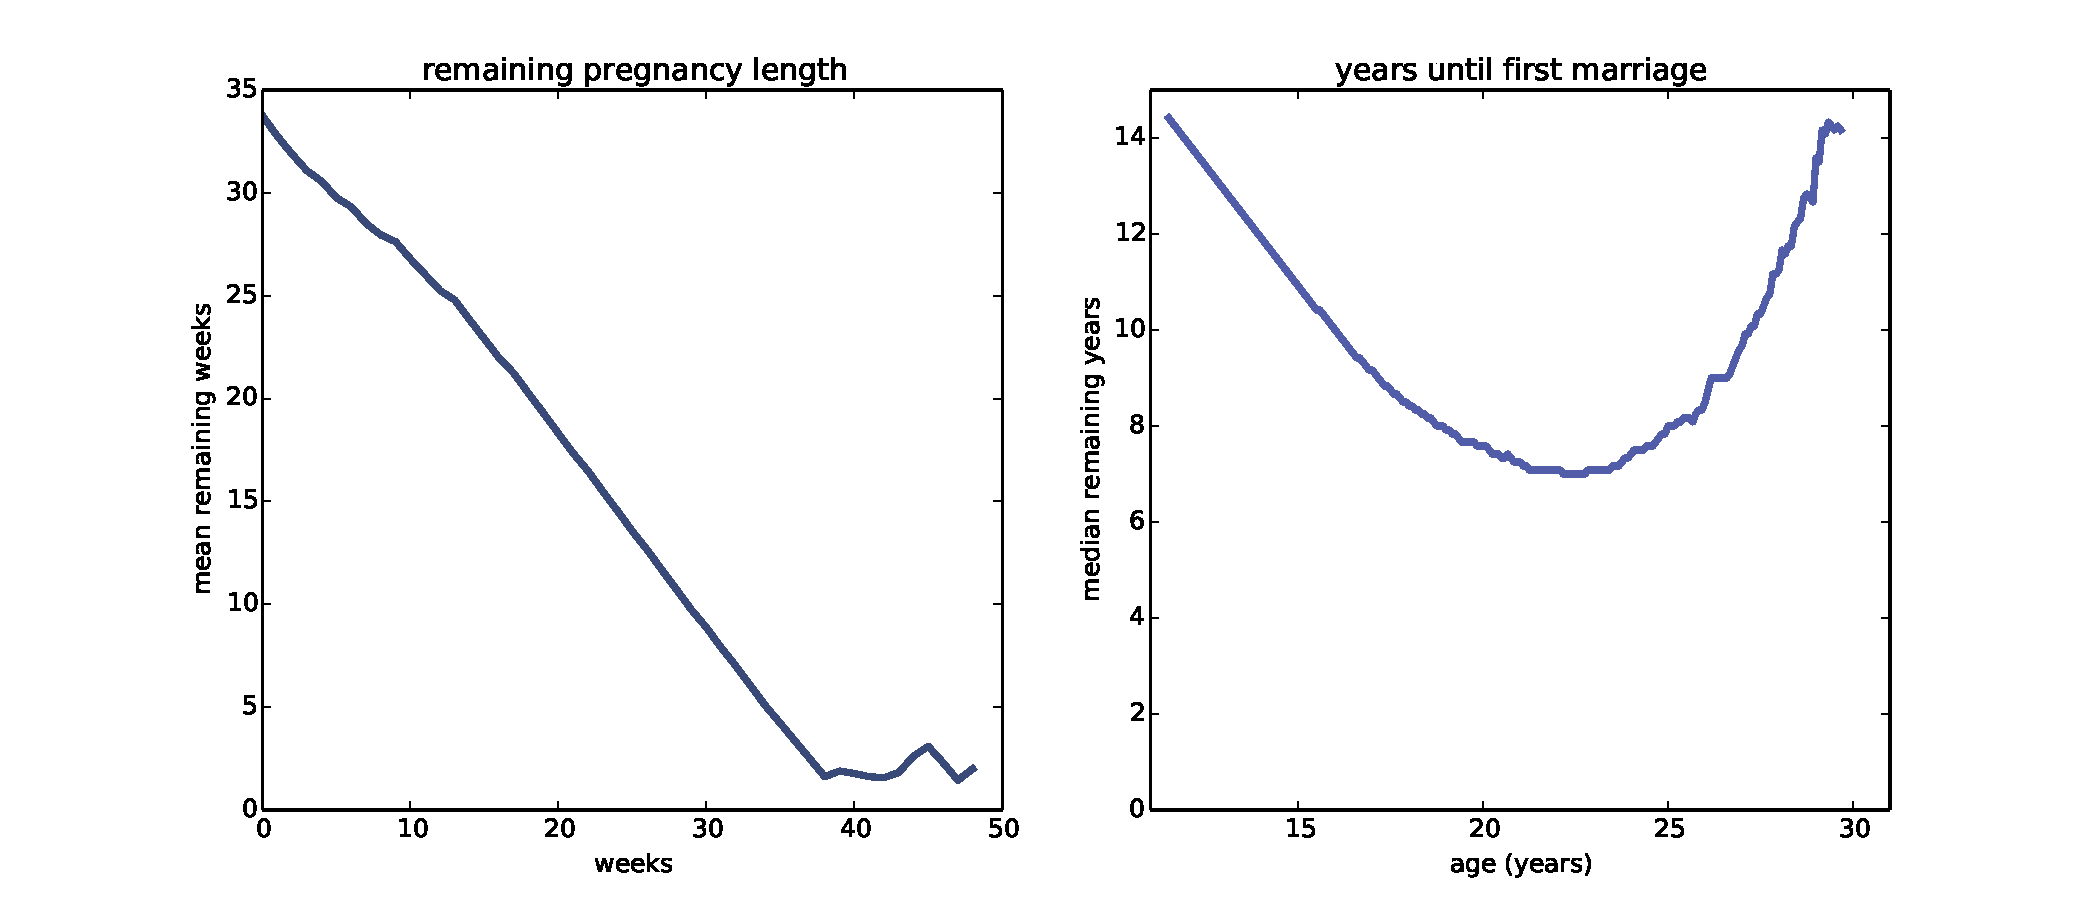
\includegraphics[height=2.5in]{figs/survival6.pdf}}
\caption{임신기간에 대한 예상 잔존여명(좌측), 초혼까지 시간(년, 우측).}
\label{survival6}
\end{figure}

그림~\ref{survival6} (왼편)에 현재 지속기간의 함수로 기대잔존임신기간이 나와 있다. 예를 들어, 0주차에는 기대잔존기간이 약 34주가 된다.
이것이 만삭(39주)보다 짧은데 이유는 임신 초기에 임신중절이 평균을 낮추기 때문이다. 
\index{임신기간 (pregnancy length)}

임신초기 기간에 곡선이 천천히 떨어진다. 13주차 뒤에는 기대잔존수명이 25주로 단지 9주만  떨어진다. 그 후에, 곡선은 주마다 약 1주씩 더 빨리 떨어진다. 

37주에서 42주 사이, 곡선은 1주와 2주 사이 수평을 유지한다. 이 기간동안 아무 시점이나 평균잔존기대수명은 같다; 매주 지나감에 따라 목표가 더이상 가까와지지 않는다. 이와 같은 특성을 가진 과정을 {\bf 무기억성(memoryless)}이라고 부른다. 이유는 과거가 예측에 아무런 효과가 없기 때문이다. 
ㅇ 행동이 산부인과 간호사의 격노하는 만트라의 수학적 기반이 된다: ``곧 지금이라도 (any day now)''
\index{무기억성 (memoryless)}

그림 ~\ref{survival6} (오른쪽)에는 연령의 함수로 초혼까지 중위수 잔존시간이 나와있다. 11살 소녀에게 초혼까지 중위수 시간은 약 14년이다. 곡선은 중위수 잔존시간이 약 7년일때 22세까지 감소한다.
그 후에 다시 올라간다: 나이 30에 시작한 연령 14년으로 다시 증가한다.

이 데이터에 기반해서, 젊은 여성은 감소하는 잔존 ``수명''을 갖는다.
이와 같은 성질을 가진 기계부품을 {\bf NBUE}(``new better than used in expectation")로 부른다. 새부품이 더 오래 갈 것으로 예상된다는 의미다.
\index{NBUE}

22세 이상되는 여성은 초혼까지 증가하는 잔존시간을 갖는다.
이와 같은 성질을 갖는 부품을 {\bf UBNE}(``used better than new in expectation'')로 부른다. 즉, 부품이 오래될수록, 더 오래 갈 것으로 예상된다. 신생아와 암환자가 또한 UBNE다; 더 오래 살수록 이들의 기대수명은 증가한다.
\index{UBNE}

이 예제에서 Cdf가 불와전해서, 평균대신에 중위수를 계산했다; 
생존곡선이 약 20\% 응답자가 44세 이전에 결혼하지 않을 것으로 추산한다. 이 여성에 대한 초혼 연령은 알려져있지 않고, 존재하지 않을지도 모른다. 그래서 평균을 계산할 수 없다.

\index{Cdf}
\index{중위수 (median)}

미지값(unknown value)을 무한대를 나타내는 특수값 {\tt np.inf}로 바꿔서 미지값을 처리한다. 이렇게 하면 모든 연령에 대해서 평균이 무한대가 된다.
하지만, 잔존수명 50\% 이상이 유한(연령 30세까지 사실이다)하기만 하면 중위수는 잘 정의된다. 이후에 유의미한 기대잔존수명을 정의하는 것은 어렵다.
\index{inf}

다음에 이들 함수를 계산하고 플롯으로 그리는 코드가 있다.

\begin{verbatim}
    rem_life1 = sf1.RemainingLifetime()
    thinkplot.Plot(rem_life1)

    func = lambda pmf: pmf.Percentile(50)
    rem_life2 = sf2.RemainingLifetime(filler=np.inf, func=func)
    thinkplot.Plot(rem_life2)
\end{verbatim}

{\tt sf1}는 임신 기간에 대한 생존함수다;
이 경우에 {\tt RemainingLifetime}에 초기설정값을 사용할 수 있다.
\index{임신기간 (pregnancy length)}

{\tt sf2}는 초혼 연령에 대한 생존함수다;
{\tt func}는 Pmf를 인자로 받아 중위수(50번째 백분위수)를 계산하는 함수다.
\index{Pmf}


\section{연습문제}

이번 연습문제에 대한 저자 해답은 \verb"chap13soln.py"에 나와있다.

\begin{exercise}

NSFG 주기 6과 7에서, {\tt cmdivorcx} 변수는 응답자의 만약 적용되다면 
년도-월(century-month)로 부호화된 첫 혼인에 대한 이혼 날짜 정보를 담고 있다.
\index{이혼}
\index{혼인상태}

이혼으로 끝나는 결혼기간과 지금까지 지속되는 혼인 기간을 계산하시오.
결혼기간에 대한 위험함수와 생존함수를 추정하시오.

표집 가중치를 고려해서 재표집을 사용하고, 표집오차를 시각화하는데
재표집으로 나온 표본에서 데이터를 도식화하시오.
\index{재표집}

응답자를 10년주기 출생으로 집단화하고, 가능하면 첫번째 혼인 연령으로 
나누는 것을 고려한다.
\index{groupby}

\end{exercise}


\section{용어 사전}

\begin{itemize}

\item 생존분석 (survival analysis): 수명, 좀더 일반적으로 사건이 일어나기까지 시간을 기술하고 예측하는 방법론 집합.
\index{생존분석 (survival analysis)}

\item 생존곡선 (survival curve): 시점 $t$에 $t$를 지나 생존 확률로 매핑하는 함수.
\index{생존곡선 (survival curve)}

\item 위험함수 (hazard function): 시점 $t$ 에 $t$ 시점까지 생존한 사람이 $t$ 시점에 사망한 비율을 매핑하는 함수.
\index{위험함수 (hazard function)}

\item 캐플란-마이어 추정 (Kaplan-Meier estimation): 위험함수와 생존함수를 추정하는 알고리즘.
\index{캐플란-마이어 추정 (Kaplan-Meier estimation)}

\item 코호트 (cohort): 특정 시간 구간에 생년월일 같은 사건으로 정의된 개체 집단.
\index{코호트 (cohort)}

\item 코호트 효과 (cohort effect): 코호트 사이 차이.
\index{코호트 효과 (cohort effect)}

\item NBUE: 기대잔존수명 성질, ``새 것이 예상하기에 오래된 것보다 좋은 것(New better than used in expectation)''
\index{NBUE}

\item UBNE: 기대잔존수명 성질, ``오래된 부품이 예상하기에 새 것보다 좋은 것(Used better than new in expectation)''
\index{UBNE}

\end{itemize}

